Na vektorovém prostoru funkcí, které jsou spojité na $[-\pi, \pi]$, můžeme definovat skalární součin:
$$\langle f \mid g \rangle = \frac{1}{\pi} \int_{-\pi}^{\pi} f(x) g(x) \dx$$

My nebudeme dokazovat, že toto je skalární součin (ani nic o Fourierových řadách, které vznikly kvůli řešení rovnic tepla a dnes jsou používány nejen při zpracování zvuku a obrazu, ale i pro analýzu časových řad, ani o cool aplikacích jako pohybový mikroskop: \url{https://www.youtube.com/watch?v=fHfhorJnAEI}).
My toto použijeme jako zajímavý typ integrálů na procvičování.

Spočítejte:
\begin{enumerate}
	
	\item  $\frac{1}{\pi} \int_{-\pi}^{\pi} \cos(mx) \cos(mx) \dx$ pro $m \in \mathbb{N}$

		\solution{
			Na minulém cvičení už jsme určili, že
			$$\int \cos^2(x) \dx = \frac{1}{2} \left( x + \sin(x)\cos(x) \right) + c $$
			Tedy jednoduchou substitucí dostaneme:
			$$\frac{1}{\pi} \int_{-\pi}^{\pi} \cos^2(mx) \dx = 1$$
		}

	\item  $\frac{1}{\pi} \int_{-\pi}^{\pi} \sin(mx) \sin(mx) \dx$ pro $m \in \mathbb{N}$

		\solution{
			Už víme, že
			$$\frac{1}{\pi} \int_{-\pi}^{\pi} \cos^2(mx) \dx = 1$$
			Navíc víme, že
			$$\frac{1}{\pi} \int_{-\pi}^{\pi} \sin^2(mx) + \cos^2(mx) \dx = \frac{1}{\pi} \int_{-\pi}^{\pi} 1 \dx = 2$$
			Tedy odvodíme:
			$$\frac{1}{\pi} \int_{-\pi}^{\pi} \sin^2(mx) \dx = 1$$
		}

	\item  $\frac{1}{\pi} \int_{-\pi}^{\pi} \cos(nx) \cos(mx) \dx$ pro $m \neq n \in \mathbb{N}$
	
		\solution{
			Použijeme vzorec, který si pamatujeme ze střední:
			$$\cos(A)\cos(B) = \frac{1}{2}\left( \cos(A - B) + \cos(A + B) \right)$$

			Napřed spočítáme primitivní funkci (mohli jsme rovnou použít pravidlo pro substituci v určitém integrálu a počítat s novými mezemi).

			Budeme volit substituci:
			\begin{align*}
				u &= (m-n)x \\
				\du &= (m-n) \dx
			\end{align*}
			respektive
			\begin{align*}
				t &= (m+n)x \\
				\dt &= (m+n) \dx
			\end{align*}
			a dostaneme:
			\begin{align*}
				\int \cos(mx) \cos(nx) \dx &= \frac{1}{2} \int \cos((m-n)x)  + \cos( (m+n)x) \dx \\
				&= \frac{1}{2} \int \cos( (m-n)x) \dx + \frac{1}{2} \int \cos( (m+n)x) \dx \\
				&= \frac{\sin( (m-n)x )}{2(m-n)} + \frac{\sin( (m+n)x )}{2(m+n)} + c
			\end{align*}

			Jelikož $\sin(ax) = -\sin(-ax)$, dostáváme že 
			$$\frac{1}{\pi} \int_{-\pi}^{\pi} \cos(mx) \cos(nx) \dx = 0$$

			Geometrický význam vidíme na
			Obrázku~\ref{fig:cosnx_cosnx} pro případ $m=n=2$
			a
			Obrázku~\ref{fig:cosmx_cosnx} pro případ $m=2, n=3$.
			\begin{figure}[H]
				\centering
				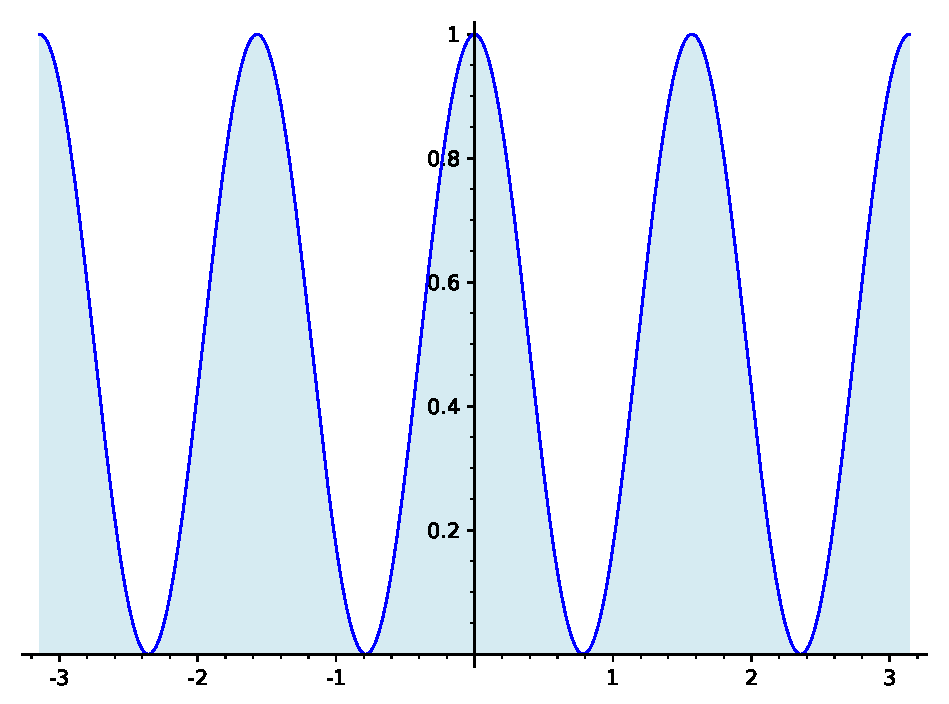
\includegraphics{cviceni_13/fig/cosnx_cosnx.pdf}
				\caption{$\frac{1}{\pi} \int_{-\pi}^{\pi} \cos(2x) \cos(2x) \dx$ tedy $m=n=2$.}
				\label{fig:cosnx_cosnx}
			\end{figure}
			\begin{figure}[H]
				\centering
				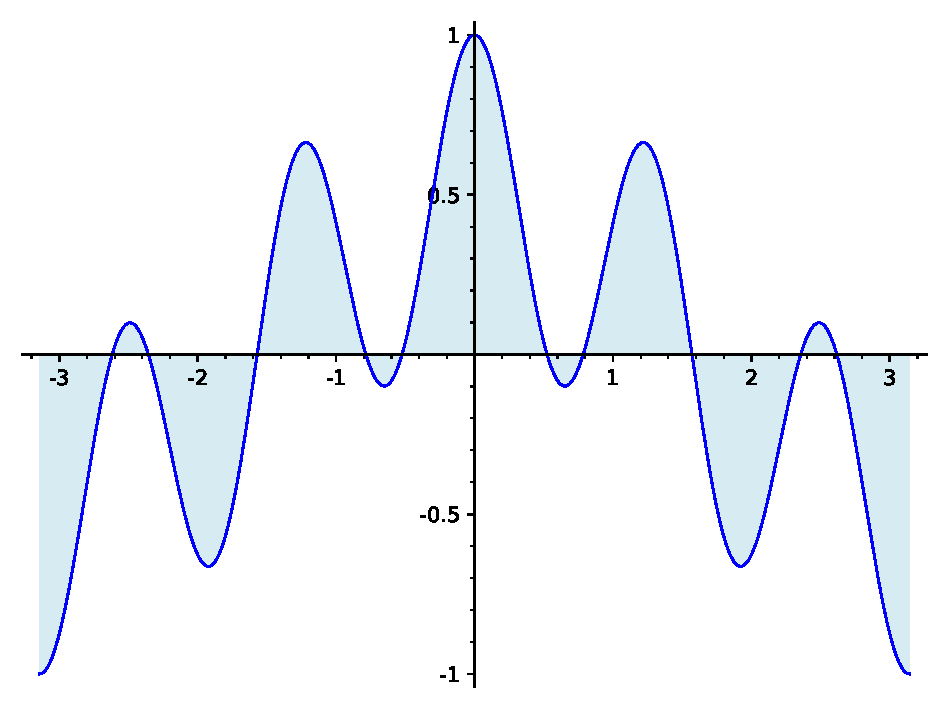
\includegraphics{cviceni_13/fig/cosmx_cosnx.pdf}
				\caption{$\frac{1}{\pi} \int_{-\pi}^{\pi} \cos(2x) \cos(3x) \dx = 0$ tedy $m=2, n=3$.}
				\label{fig:cosmx_cosnx}
			\end{figure}
		
			Poznamenejme, že stejný výsledek dostanete i pro součin dvou sinů $\langle \sin(mx) \mid \sin(nx) \rangle$ -- vyzkoušejte.
		}
	
	\item  $\frac{1}{\pi} \int_{-\pi}^{\pi} \sin(nx) \cos(mx) \dx$ pro $m, n \in \mathbb{N}$

		\solution{
			Použijeme podobný trik jako minule:
			$$\sin(A)\cos(B) = \frac{1}{2}\left( \sin(A + B) + \sin(A - B) \right)$$
			a dostaneme (jako cvičení si dopočítejte mezikroky):
			$$\frac{1}{\pi} \int_{-\pi}^{\pi} \sin(nx) \cos(mx) \dx = 0$$
			
			Obrázek~\ref{fig:sin2x_cos3x} ukazuje situaci pro případ $m=3, n=2$.
			\begin{figure}[H]
				\centering
				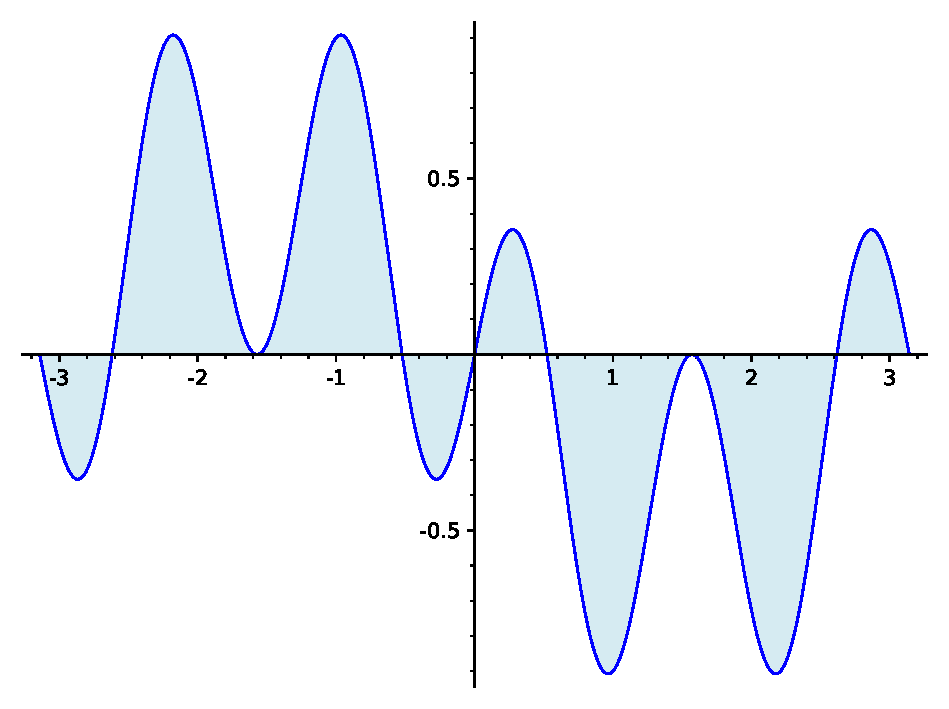
\includegraphics{cviceni_13/fig/sin2x_cos3x.pdf}
				\caption{$\frac{1}{\pi} \int_{-\pi}^{\pi} \sin(2x) \cos(3x) \dx = 0$.}
				\label{fig:sin2x_cos3x}
			\end{figure}
		}

	\item  Pro funkci $s(x) = x / \pi$ na $[-\pi, \pi]$ která je navíc periodická s periodou $2\pi$ (tzn. $\forall x \in \mathbb{R} \colon s(x) = s(x + 2\pi)$) spočítejte:

		\begin{enumerate}

			\item  $a_n = \frac{1}{\pi} \int_{\pi}^{\pi} s(x) \cos(nx) \dx$ pro $n \in \mathbb{N} \cup \left\{ 0 \right\}$

				\solution{
					Funkce je lichá a integrujeme na intervalu symetrickém okolo nuly, tedy
					$$a_n = \frac{1}{\pi} \int_{\pi}^{\pi} s(x) \cos(nx) \dx = 0$$
				}
			
			\item  $b_n = \frac{1}{\pi} \int_{\pi}^{\pi} s(x) \sin(nx) \dx$ pro $n \in \mathbb{N}$

				\solution{
					Na intervalu $[-\pi, \pi]$ je $s(x) = x / \pi$.
					Naštěstí už jsme v minulých cvičeních spočítali, že
					$$\int x \sin(x) \dx = -x \cos(x) + \sin(x) + c$$
					teď už stačí použít jednoduchou substituci (dopočítejte).

					Tedy dostáváme, že
					$$b_n = \frac{1}{\pi} \int_{\pi}^{\pi} s(x) \cos(nx) \dx = \frac{2(-1)^{n+1}}{\pi n}$$
					pro $n \geq 1$.
				}

			\item  Co se stane, když sečteme prvních několik členů následující řady:
				$$\frac{a_0}{2} + \sum_{n = 1}^{\infty} \left( a_n \cos(nx) + b_n \sin(nx) \right)$$

				\solution{
					Dostaneme \uv{aproximaci} původní funkce pomocí součtu sinů a cosinů.
					Příklad pro $n=5$ je na Obrázku~\ref{fig:fourierova_rada}.
					\begin{figure}[H]
						\centering
						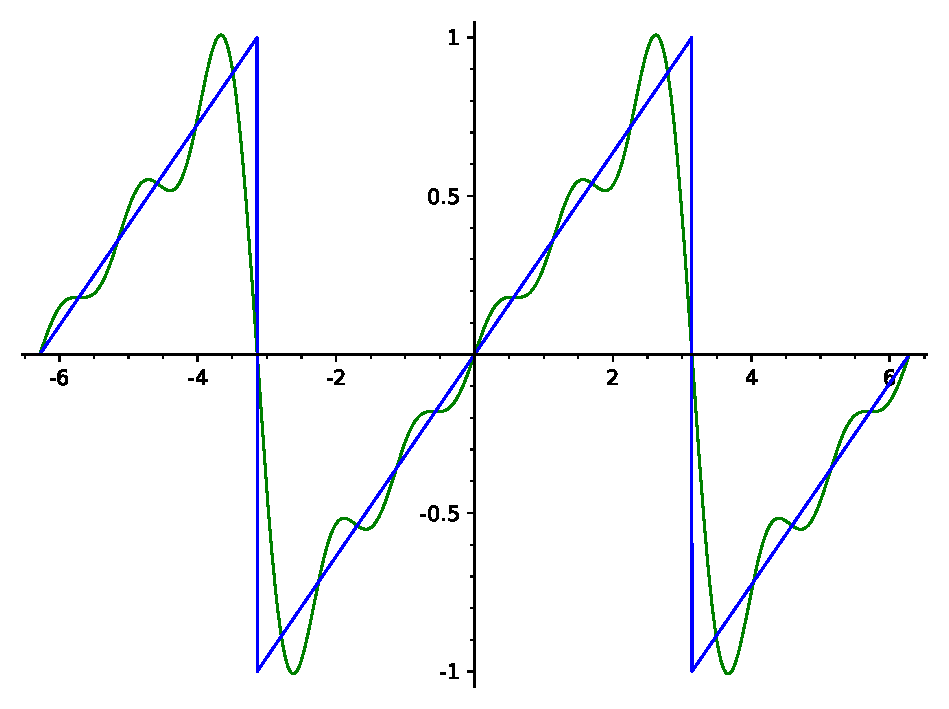
\includegraphics{cviceni_13/fig/fourierova_rada.pdf}
						\caption{Součet prvních pár členů Fourierovy řady pro $s(x)$.}
						\label{fig:fourierova_rada}
					\end{figure}
				}

		\end{enumerate}

\end{enumerate}

